
The Fourier Volume Reconstruction (FVR) method described in sections \ref{Sec:VolumeRegistrationSection} and \ref{Sec:AFVRApproach} were designed to be independent of RGB-D information input and thus sensors. As long as greyscale data with a depth component, RGB data with a depth component or depth data on their own are input, the FVR method should be able to compute accurate relative dense 3D reconstructions and optionally relative camera pose data. This section details both RGB-D sensor input advantages and disadvantages as well as those for monocular video input. Input via a stereo setup is also discussed. However, since there is much research on stereo methods which often reach accuracy which approaches RGB-D sensors, more focus is given to depth sensor based input as well as monocular video input, which is the most difficult data to work with. \\

\subsubsection{Depth Sensor Based Reconstruction}

Depth sensor input is advantageous for several reasons. It is faster than both stereo and monocular methods, and has more robustness and reliability. In general, it is also more accurate than stereo methods, and in most cases is more accurate than monocular based methods. The major disadvantage in using such sensors has historically been one of accessibility. Thanks to systems such as the Microsoft Kinect and the Asus Xtion Pro Live camera being available to the general public at a low expense, this is changing. However, there is still a mass of legacy video data which does not have actively generated depth data provided, moreover there is still a wealth of content still being produced by simple RGB cameras. \\

Another drawback of this method is that of accuracy. The accuracy of both the Kinect and Asus Xtion Pro Live sensors is limited to the resolution of the device. To alleviate this, some sub-pixel resolution generating algorithms may be used. These methods can be used in an attempt to generate greater resolution for given depth data. Methods may work on frames in a standalone fashion, although additional data such as consecutive frames and multi-camera techniques may also be used. Both the Microsoft Kinect and Asus Xtion Live Pro have maximum resolutions of $640 \times 480$. Methods of depth generation based on stereo data input (as well as monocular input) are capable of generating dense depth information at resolutions only limited by the resolution of the cameras used. As of 2017, most cameras, even those found on mobile devices, can generate video data at resolutions of $1024 \times 1080$. \\

Another possible drawback in using RGB-D sensors is that certain materials reflect the infra-red light used by such active cameras to compute the depth information. These sensors are also known to produce noise depth data around the corners and edges of objects captured within the frame. Since most computer vision algorithms make use of such salient features such as edges and corners within the image data, this can lead to inaccurate 3D reconstructions, especially in cases where 2D feature matching is used with RANSAC to produce 3D camera pose information. These sensors are also limited to indoor environments, their infra-red sensor components are saturated in the sunlight, and therefore little to no useful depth data may be generated in full sunlight. This is a major drawback as much of the world is made up of complex outdoor environments, therefore this is an unfortunate restriction given the usefulness of such cameras in indoor environments and lower light environments. \\

Another major disadvantage is that these sensors cannot produce depth data over distances. This is to do with the range of the active infra-red projection component of these sensors. Because the projection cannot reach far distances, the infra-red sensor cannot detect depth. This is in contrast to stereo and monocular methods which are capable of distant depth estimates.  

RGB-D camera sensors are still a popular choice for 3D reconstruction frameworks as the depth data produced by these methods is faster and more reliable than other sensors and techniques. For scenes and environments which can be accurately scanned by such depth sensors (such as environments with low sunlight, short ranges as in office environments and scenes with few objects which reflect infra-red light), RGB-D cameras are typically the preferred choice. The RGB-D data used to test the FVR method comes from an Asus Xtion Pro LIVE sensor. This sensor produces a colour and depth image input pair, which is processed in order to generate 3D volume frames which are the required input to the FVR method. \\

The color and depth image pair are referred to by $f(u,v)$ and $g(u,v)$, $f(u,v)$ refers to the color image and $g(u,v)$ refers to the depth image. The colour image data contains a reg, green and blue component each between the range $[0,255]$. Depth information is processed within the range $[0,10000]$. In terms of resolution, $u$ ranges $[0..639]$ and $v$ ranges $[0..479]$ giving a resolution of $640 \times 480$. Examples of images generated by the Asus Xtion Pro LIVE sensor are shown in figures \ref{fig:COLEXAMPLE} and \ref{fig:DEPTHEXAMPLE}. Using $Z_{u,v}$ = $g(u,v)$, $f(u,v)$ is projected into 3D space using equation \ref{eqn:PC_PROJECTION} to obtain the $X_{u,v}$ and $Y_{u,v}$ coordinate values in 3D space. Here, $c_x$ and $c_y$ represent the intersection point where the optical axis intersects the projection plane and are defined as $c_x = 319.5$, $c_y = 239.5$. Also $f_x$ and $f_y$ represent the focal length which is defined as $f_x$, $f_y = 525.0$. \\


\begin{equation} \label{eqn:PC_PROJECTION}
\begin{split}
X_{u,v} & = \frac{(u - c_x)Z_{u,v}}{f_x} \\
Y_{u,v} & = \frac{(v - c_y)Z_{u,v}}{f_y} \\
\end{split}
\end{equation}

\begin{figure}[!htb] 
        \centering
        \begin{subfigure}[b]{1.8in}
                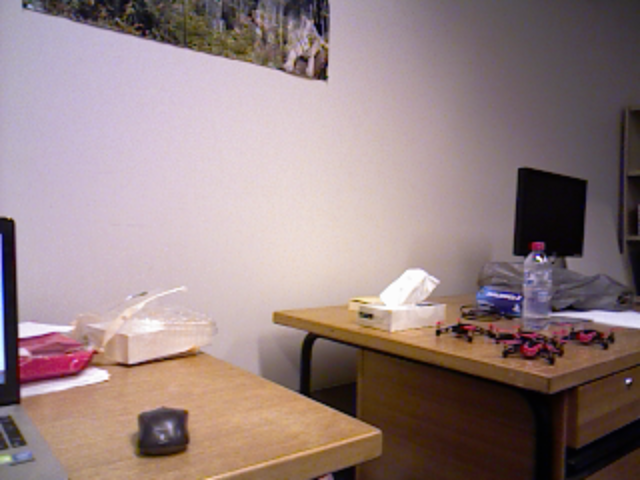
\includegraphics[width=1.7in]{images/ch2/colorF11}
                \caption{Color Image}
                \label{fig:COLEXAMPLE}
        \end{subfigure}%
        \begin{subfigure}[b]{1.8in}
                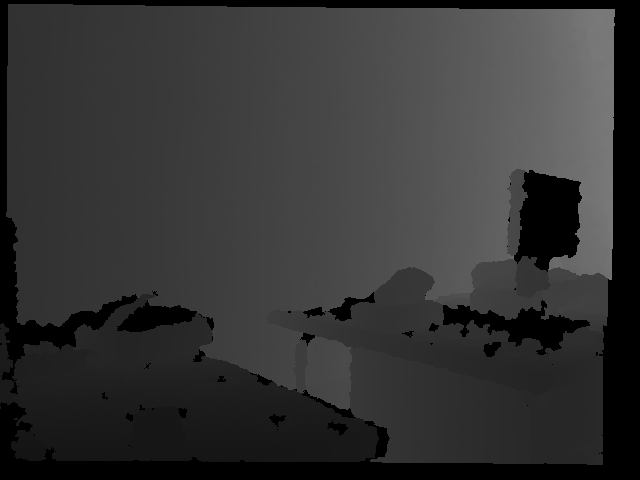
\includegraphics[width=1.7in]{images/ch2/depthF11}
                \caption{Depth Image}
                \label{fig:DEPTHEXAMPLE}
        \end{subfigure}
        
         \begin{subfigure}[b]{1.8in}
                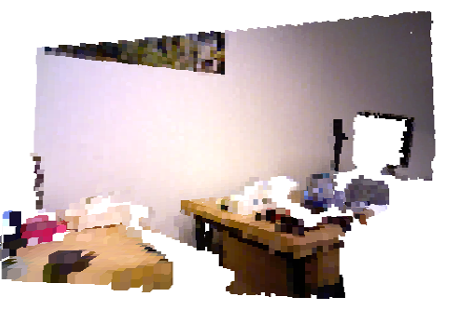
\includegraphics[width=1.8in]{images/ch2/volumeF11128}
                \caption{Projected Volume $128^3$}
                \label{fig:VOLUMEEXAMPLE128}
        \end{subfigure}%
         \begin{subfigure}[b]{1.8in}
                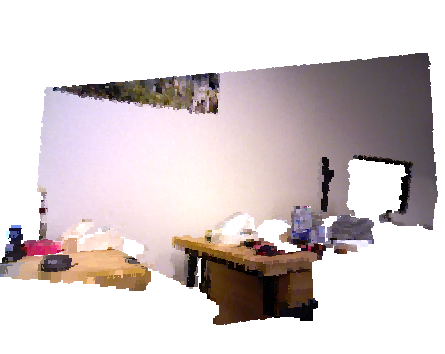
\includegraphics[width=1.8in]{images/ch2/volumeF11256}
                \caption{Projected Volume $256^3$}
                \label{fig:VOLUMEEXAMPLE384}
        \end{subfigure}%
       \caption{A Projected Frame.}
       \label{fig:PROJECTED_FRAME}
\end{figure}


To facilitate further processing, the projected image volumes are re-sampled. The results reported in this paper were obtained using volumes of $256^3$ voxels in size. An example colour and depth image pair and their volumetric projection is shown in figure \ref{fig:PROJECTED_FRAME}.  \\


\subsubsection{Stereo Camera Based Reconstruction}

The Fourier volume registration methods also work with stereo camera based data. This information can be generated using several of the techniques described in the literature review. Essentially the data must then be projected into depth frames which are registered using one of the proposed fourier volume registration techniques. Because stereo methods do not always accurately compute depth to scale, fourier volume registration has an advantage over other methods in that it also registers against scale. For systems where depth is estimated accurately (as accurately or more than depth sensors) results should work similarly.

\subsubsection{Monocular Sensor Based 3D Reconstruction}

Some preliminary research has been conducted in evaluating the use of Fourier volume registration given monocular data. From monocular video frames, depth was first computed. This data was fed into the fourier volume registration method in computing 3D reconstructions. Preliminary results are presented but further investigation is required in this area.

